%<dscrpt>Fichier de déclarations Latex à inclure au début d'un élément de cours.</dscrpt>

\documentclass[a4paper]{article}
\usepackage[hmargin={1.8cm,1.8cm},vmargin={2.4cm,2.4cm},headheight=13.1pt]{geometry}

%includeheadfoot,scale=1.1,centering,hoffset=-0.5cm,
\usepackage[pdftex]{graphicx,color}
\usepackage[french]{babel}
%\selectlanguage{french}
\addto\captionsfrench{
  \def\contentsname{Plan}
}
\usepackage{fancyhdr}
\usepackage{floatflt}
\usepackage{amsmath}
\usepackage{amssymb}
\usepackage{amsthm}
\usepackage{stmaryrd}
\usepackage{ucs}
\usepackage[utf8]{inputenc}
%\usepackage[latin1]{inputenc}
\usepackage[T1]{fontenc}


\usepackage{titletoc}
%\contentsmargin{2.55em}
\dottedcontents{section}[2.5em]{}{1.8em}{1pc}
\dottedcontents{subsection}[3.5em]{}{1.2em}{1pc}
\dottedcontents{subsubsection}[5em]{}{1em}{1pc}

\usepackage[pdftex,colorlinks={true},urlcolor={blue},pdfauthor={remy Nicolai},bookmarks={true}]{hyperref}
\usepackage{makeidx}

\usepackage{multicol}
\usepackage{multirow}
\usepackage{wrapfig}
\usepackage{array}
\usepackage{subfig}


%\usepackage{tikz}
%\usetikzlibrary{calc, shapes, backgrounds}
%pour la présentation du pseudo-code
% !!!!!!!!!!!!!!      le package n'est pas présent sur le serveur sous fedora 16 !!!!!!!!!!!!!!!!!!!!!!!!
\usepackage[french,ruled,vlined]{algorithm2e}

%pr{\'e}sentation du compteur de niveau 2 dans les listes
\makeatletter
\renewcommand{\labelenumii}{\theenumii.}
\renewcommand{\thesection}{\Roman{section}.}
\renewcommand{\thesubsection}{\arabic{subsection}.}
\renewcommand{\thesubsubsection}{\arabic{subsubsection}.}
\makeatother


%dimension des pages, en-t{\^e}te et bas de page
%\pdfpagewidth=20cm
%\pdfpageheight=14cm
%   \setlength{\oddsidemargin}{-2cm}
%   \setlength{\voffset}{-1.5cm}
%   \setlength{\textheight}{12cm}
%   \setlength{\textwidth}{25.2cm}
   \columnsep=1cm
   \columnseprule=0.5pt

%En tete et pied de page
\pagestyle{fancy}
\lhead{MPSI-\'Eléments de cours}
\rhead{\today}
%\rhead{25/11/05}
\lfoot{\tiny{Cette création est mise à disposition selon le Contrat\\ Paternité-Pas d'utilisations commerciale-Partage des Conditions Initiales à l'Identique 2.0 France\\ disponible en ligne http://creativecommons.org/licenses/by-nc-sa/2.0/fr/
} }
\rfoot{\tiny{Rémy Nicolai \jobname}}

\newcommand{\baseurl}{http://back.maquisdoc.net/data/cours\_nicolair/}
\newcommand{\urlexo}{http://back.maquisdoc.net/data/exos_nicolair/}

\newcommand{\N}{\mathbb{N}}
\newcommand{\Z}{\mathbb{Z}}
\newcommand{\C}{\mathbb{C}}
\newcommand{\R}{\mathbb{R}}
\newcommand{\D}{\mathbb{D}}
\newcommand{\K}{\mathbf{K}}
\newcommand{\Q}{\mathbb{Q}}
\newcommand{\F}{\mathbf{F}}
\newcommand{\U}{\mathbb{U}}
\newcommand{\p}{\mathbb{P}}


\newcommand{\card}{\mathop{\mathrm{Card}}}
\newcommand{\Id}{\mathop{\mathrm{Id}}}
\newcommand{\Ker}{\mathop{\mathrm{Ker}}}
\newcommand{\Vect}{\mathop{\mathrm{Vect}}}
\newcommand{\cotg}{\mathop{\mathrm{cotan}}}
\newcommand{\sh}{\mathop{\mathrm{sh}}}
\newcommand{\ch}{\mathop{\mathrm{ch}}}
\newcommand{\argsh}{\mathop{\mathrm{argsh}}}
\newcommand{\argch}{\mathop{\mathrm{argch}}}
\newcommand{\tr}{\mathop{\mathrm{tr}}}
\newcommand{\rg}{\mathop{\mathrm{rg}}}
\newcommand{\rang}{\mathop{\mathrm{rg}}}
\newcommand{\Mat}{\mathop{\mathrm{Mat}}}
\renewcommand{\Re}{\mathop{\mathrm{Re}}}
\renewcommand{\Im}{\mathop{\mathrm{Im}}}
\renewcommand{\th}{\mathop{\mathrm{th}}}
\newcommand{\repere}{$(O,\overrightarrow{i},\overrightarrow{j},\overrightarrow{k})$}
\newcommand{\cov}{\mathop{\mathrm{Cov}}}

\newcommand{\absolue}[1]{\left| #1 \right|}
\newcommand{\fonc}[5]{#1 : \begin{cases}#2 \rightarrow #3 \\ #4 \mapsto #5 \end{cases}}
\newcommand{\depar}[2]{\dfrac{\partial #1}{\partial #2}}
\newcommand{\norme}[1]{\left\| #1 \right\|}
\newcommand{\se}{\geq}
\newcommand{\ie}{\leq}
\newcommand{\trans}{\mathstrut^t\!}
\newcommand{\val}{\mathop{\mathrm{val}}}
\newcommand{\grad}{\mathop{\overrightarrow{\mathrm{grad}}}}

\newtheorem*{thm}{Théorème}
\newtheorem{thmn}{Théorème}
\newtheorem*{prop}{Proposition}
\newtheorem{propn}{Proposition}
\newtheorem*{pa}{Présentation axiomatique}
\newtheorem*{propdef}{Proposition - Définition}
\newtheorem*{lem}{Lemme}
\newtheorem{lemn}{Lemme}

\theoremstyle{definition}
\newtheorem*{defi}{Définition}
\newtheorem*{nota}{Notation}
\newtheorem*{exple}{Exemple}
\newtheorem*{exples}{Exemples}


\newenvironment{demo}{\renewcommand{\proofname}{Preuve}\begin{proof}}{\end{proof}}
%\renewcommand{\proofname}{Preuve} doit etre après le begin{document} pour fonctionner

\theoremstyle{remark}
\newtheorem*{rem}{Remarque}
\newtheorem*{rems}{Remarques}

\renewcommand{\indexspace}{}
\renewenvironment{theindex}
  {\section*{Index} %\addcontentsline{toc}{section}{\protect\numberline{0.}{Index}}
   \begin{multicols}{2}
    \begin{itemize}}
  {\end{itemize} \end{multicols}}


%pour annuler les commandes beamer
\renewenvironment{frame}{}{}
\newcommand{\frametitle}[1]{}
\newcommand{\framesubtitle}[1]{}

\newcommand{\debutcours}[2]{
  \chead{#1}
  \begin{center}
     \begin{huge}\textbf{#1}\end{huge}
     \begin{Large}\begin{center}Rédaction incomplète. Version #2\end{center}\end{Large}
  \end{center}
  %\section*{Plan et Index}
  %\begin{frame}  commande beamer
  \tableofcontents
  %\end{frame}   commande beamer
  \printindex
}


\makeindex
\begin{document}
 %pour compiler avec algoritm2e
% attention utilise \usepackage[french,ruled,vlined]{algorithm2e} alors que le package n'est pas présent sur le serveur svn le pdf. Le pdf est ajouté à svn.
\debutcours{Arithmétique polynômiale}{ 0.4 \tiny{ le \today}}


La partie du programme intitulée \og Polynômes et fractions rationnelles\fg~ est présentée dans trois documents distincts \href{\baseurl C1622.pdf}{Polynômes}, \href{\baseurl C2160.pdf}{Arithmétique polynomiale} (ce document)  et \href{\baseurl C1623.pdf}{Fractions rationnelles}.

\section{Divisibilité}
\subsection{Définitions}
\begin{prop}[Inversibles]
 L'ensemble des éléments inversibles de $\K[X]$ est $\K_0[X]\setminus\{0_{\K[X]}\}$ (ensemble des polynômes de degré $0$).
\end{prop}
\begin{defi}
 Soit $A$ et $B$ dans $\K[X]$. On dit que $A$ divise $B$ si et seulement si il existe $C\in \K[X]$ tel que $B=CA$. On dit aussi alors que $B$ est un multiple de $A$. 
\end{defi}
\begin{nota}
  Soit $A\in \K[X]$ un polynôme. On désigne par $\mathcal D (A)$ l'ensemble des diviseurs de $A$ et par $\mathcal M (A)$ l'ensemble de ses multiples. 
\end{nota}
\begin{rems}
\begin{enumerate}
 \item Avec cette définition $\mathcal{D}(0) = \K[X]$.
 \item Soit $A$ et $B$ deux polynômes, alors $\mathcal M (A)\cap \mathcal M (B)$ est l'ensemble des multiples communs à $A$ et $B$ et $\mathcal D (A)\cap \mathcal D (B)$ est l'ensemble des diviseurs communs à $A$ et $B$. 
 \item Soit $A$ et $B$ deux polynômes non nuls,
\[
 A \text{ divise } B \Rightarrow \deg(A) \leq \deg(B), \hspace{0.5cm} A \text{ multiple de } B \Rightarrow \deg(A) \geq \deg B. 
\]
\end{enumerate} 
\end{rems}

\index{polynômes associés}
\begin{defi}
 Deux polynômes non nuls sont dits \emph{associés} si et seulement si ils sont égaux à la multiplication près par un élément non nul du corps.
\end{defi}
Deux polynômes non nuls $A$ et $B$ sont associés si et seulement si il existe $\lambda \in \K^*$ tel que $B=\lambda A$.
\begin{prop}
 Soit $A$ et $B$ deux polynômes non nuls, alors
\[
 A \text{ et } B \text{ associés} \Leftrightarrow A \text{ et } B \text{ se divisent mutuellement}
\Leftrightarrow A \text{ et } B \text{ multiples l'un de l'autre.}
\]
\end{prop}
\begin{demo}
 à compléter
\end{demo}

\begin{rem}
  \begin{enumerate}
       \item  Soit $A$ et $B$ deux polynômes non nuls. Alors $\mathcal M (A)=\mathcal M (B)$ ou  $\mathcal D (A)=\mathcal D (B)$ si et seulement si $A$ et $B$ sont égaux à multiplication près par un élément non nul du corps des coefficients.
       \item Considérons une famille de polynômes de la forme $\lambda A$ où $A$ est un polynôme fixé et $\lambda$ un élément non nul quelconque de $K$. Il existe un seul polynôme unitaire dans cette famille. En général on choisit ce polynôme unitaire pour représenter la famille.
   \end{enumerate}
\end{rem}


\subsection{PPCM.}
\index{plus petit commun multiple ppcm}
\begin{defi}
 Soit $A$ et $B$ deux polynômes non nuls.  L'ensemble des degrés des polynômes non nuls de $\mathcal{M}(A)\cap \mathcal{M}(B)$ est une partie non vide de $\N$. Elle admet un plus petit élément. Un \emph{plus petit commun multiple} (ppcm) de $A$ et $B$ est un polynôme de $\mathcal{M}(A)\cap \mathcal{M}(B)$ dont le degré est égal à ce plus petit élément. Un ppcm est donc un polynôme de degré minimal parmi les multiples communs non nuls.
\end{defi}

\begin{nota}
 Soit $A$ et $B$ deux polynômes non nuls, un ppcm est noté $A\vee B$ ou simplement $\text{ppcm}(A,B)$.
\end{nota}

\begin{prop}
Soit $A$ et $B$ deux polynômes non nuls et $M$ un ppcm de $A$ et $B$. Alors  $\mathcal{M}(A)\cap \mathcal{M}(B) = \mathcal{M}(M)$.
\end{prop}
\begin{demo}
Par définition, $\mathcal{M}(M) \subset \mathcal{M}(A) \cap \mathcal{M}(B)$. Réciproquement, si $P$ est un multiple commun non nul, divisons le par $M$. Il existe des polynômes $Q$ et $R$ avec $\deg(R) < \deg(M)$ tel que $P = QM +R$. Comme $P$ et $Q$ sont  des multiples communs, $R = P-QM$ aussi. La minimalité du degré de $M$ entraine alors que $R=0$ ce qui prouve
\[
 \mathcal{M}(A)\cap \mathcal{M}(B) \subset \mathcal{M}(M). 
\]
\end{demo}
\begin{rem}
 On déduit de la proposition précédente que, si $M_1$ et $M_2$ sont deux ppcm de $A$ et $B$ alors $\mathcal{M}(M_1)=\mathcal{M}(M_2)$. Les ppcm sont donc associés entre eux.\newline
 Il existe un unique ppcm de $A$ et $B$ unitaire.
\end{rem}
On peut étendre la définition du ppcm aux familles de $m$ polynômes $(A_1, \cdots, A_m)$ non nuls. Il existe des multiples communs non nuls de degré minimal. Un tel polynôme est appelé ppcm de la famille (noté $A_1 \vee \cdots \vee A_m$). Il vérifie
\[
 \mathcal{M}(A_1) \cap \cdots \cap \mathcal{M}(A_m) = \mathcal{M}(A_1 \vee \cdots \vee A_m).
\]
Comme l'intersection est associative, l'opération $\vee$ l'est aussi (à multilplication près par un élément non nul du corps).
Linéarité du ppcm à compléter

\subsection{PGCD}
\subsubsection{Algorithme d'Euclide}
\index{plus grand diviseur commun pgcd}
\begin{defi}
 Soit $A$ et $B$ deux polynômes non nuls. L'ensemble des degrés des polynômes de $\mathcal{D}(A)\cap \mathcal{D}(B)$ est une partie de $\N$ majorée par $\min(\deg(A),\deg(B))$. Elle admet donc un plus grand élément. Un \emph{plus grand commun dénominateur} (pgcd) de $A$ et $B$ est un diviseur commun dont le degré est ce plus grand élément. Un pgcd est un diviseur commun  de degré maximal.
\end{defi}

\begin{nota}
 Soit $A$ et $B$ deux polynômes non nuls. Un pgcd de $A$ et $B$ est noté $A\wedge B$ ou simplement $\text{pgcd}(A,B)$.
\end{nota}

\index{pgcd! calcul}
\begin{algorithm}
 $A\leftarrow$ un polynôme $A_0$\;
 $AA\leftarrow$ un polynôme non nul $A_1$\;
 \Tq{$AA \neq 0$}{
   $A, AA \leftarrow AA$, reste de la division de $A$ par $AA$\;
 }
 renvoyer $A$\;
 \caption{Calcul du pgcd}
 \label{algopgcd}
\end{algorithm}

\begin{prop}
Soit $A_0$ et $A_1$ deux polynômes non nuls et $D$ le polynôme renvoyé par l'algorithme d'Euclide (algorithme \ref{algopgcd}) initialisé par $A_0$ et $A_1$. Alors  $\mathcal{D}(A)\cap \mathcal{D}(B) = \mathcal{D}(D)$ et $D$ est un pgcd de $A_0$ et $A_1$.
\end{prop}
\begin{demo}
 La boucle de l'algorithme se termine car le degré de $AA$ est une fonction de terminaison. L'égalité
\[
 \mathcal{D}(A) \cap \mathcal{D}(AA) =  \mathcal{D}(A_0) \cap \mathcal{D}(A_1)
\]
est un invariant de la boucle. Après la sortie de la boucle on a donc
\[
 \mathcal{D}(A_0) \cap \mathcal{D}(A_1) = \mathcal{D}(A) \cap \mathcal{D}(AA) = \mathcal{D}(A) \cap \mathcal{D}(0) = \mathcal{D}(A).
\]
Notons $D$ la valeur de $A$ renvoyée par l'algorithme. La relation sur les ensembles de diviseurs entraine la maximalité du degré de $D$ parmi les degrés des diviseurs communs. C'est donc un pgcd.
\end{demo}
\begin{prop}
 Soit $A_0$ et $A_1$ deux polynômes non nuls et $D_1$ un pgcd de $A_0$ et $A_1$. Il est alors associé au pgcd renvoyé par l'algorithme d'Euclide. En particulier, tous les pgcd sont associés entre eux.
\end{prop}
\begin{demo}
 Soit $D$ le polynôme renvoyé par l'algorithme d'Euclide. Comme $\mathcal{D}(A_0)\cap\mathcal{D}(A_1)=\mathcal{D}(D)$, on sait que $D_1\in \mathcal{D}(D)$donc $D_1$divise $D$. Il existe un polynôme $C$ tel que $D = CD_1$. Or par définition des pgcd avec le degré, $D$ et $D_1$ sont de même degré donc $\deg(C)=0$ c'est à dire que $C$ est un élément non nul du corps. Les polynômes $D$ et $D_1$ sont associés. Deux pgcd quelconques sont associésentre eux car il sont associés à $D$.
\end{demo}
Avec la remarque sur le fait que les pgcd sont associés, on note alors $A\wedge B = 1$.
\begin{rem}
 Il existe un unique pgcd unitaire. Il peut être utile de le choisir mais ce n'est pas toujours le cas.
\end{rem}

\index{polynômes premiers entre eux}
\begin{defi}
 Deux polynômes non nuls sont dits \emph{premiers entre eux} si et seulement si les pgcd sont de degré $0$.
\end{defi}
\begin{rem}
 Deux polynômes non nuls sont premiers entre eux si et seulement si les polynômes de degré $0$ sont leurs seuls diviseurs communs. 
\end{rem}


On peut étendre la définition du pgcd aux familles de $m$ polynômes $(A_1, \cdots, A_m)$ non nuls. Il existe des diviseurs communs de degré maximal. Un tel polynôme est appelé pgcd de la famille (noté $A_1 \wedge \cdots \wedge A_m$). Il vérifie
\[
 \mathcal{D}(A_1) \cap \cdots \cap \mathcal{D}(A_m) = \mathcal{D}(A_1 \vee \cdots \vee A_m).
\]
Comme l'intersection est associative, l'opération $\wedge$ l'est aussi (à multilplication près par un élément non nul du corps).

\subsubsection{Coefficients complexes et racines communes.}
Dans $\C[X]$, tout polynôme de degré au moins $1$ admet des racines. On en déduit:
\begin{prop}
 Soit $A$ et $B$ deux polynômes non nuls de $\C[X]$.
\[
 \deg(A\wedge B) \geq 1 \Leftrightarrow A \text{ et } B \text{ ont des racines communes.}
\]
\end{prop}
\begin{demo}
 Si $\deg(A\wedge B) \geq 1$, $\deg(A\wedge B)$ admet au moins une racine $z$. Le polynôme $X-z$ divise $A\wedge B$ donc il divise $A$ et $B$ donc $z$ est une racine commune à $A$ et $B$.\newline
 Réciproquement, si $A$ et $B$ ont une racine $z$ en commun, alors le polynôme $X-z$ est un diviseur commun donc $\deg(A\wedge B)\geq 1$.
\end{demo}

\begin{rem}
 Soit $A\in \C[X]$ avec $\deg(A)\geq 2$. Alors $A$ admet au moins une racine multiple si et seulement si $\deg(A\wedge A') \geq 1$. Ou encore: 
\[
 A \text{ n'admet que des racines simples } \Leftrightarrow A \wedge A' = 1 \Leftrightarrow A \text{ et } A' \text{ premiers entre eux}.
\]
\end{rem}

\subsection{Théorème de Bezout.}
\subsubsection{Algorithme d'Euclide étendu.}
\index{algorithme d'Euclide étendu}
\begin{algorithm}
  $A\leftarrow$ un polynôme $A_0$\;
  $AA\leftarrow$ un polynôme non nul $A_1$\;
  $U\leftarrow 1$\;
  $UU\leftarrow 0$\;
  $V\leftarrow 0$\;
  $VV\leftarrow 1$\;
  \Tq{$AA \neq 0$}{
    
    $Q \leftarrow $ quotient de la division de $A$ par $AA$\;
    \;
    $AAA \leftarrow A - Q*AA$\;
    $UUU \leftarrow U - Q*UU$\;
    $VVV \leftarrow V - Q*VV$\;
    \;
    $U \leftarrow UU$\;
    $UU \leftarrow UUU$\;
    \;
    $V \leftarrow VV$\;
    $VV \leftarrow VVV$\;
    \;
    $A \leftarrow AA$\;
    $AA \leftarrow AAA$\;
  }
  renvoyer $A, U, V$\;
 \caption{Euclide étendu}
 \label{algoEucEtend}
\end{algorithm}

\begin{prop}
 Soit $A_0$, $A_1$ deux polynômes non nuls et $D$, $U$, $V$ les polynômes renvoyés par l'algorithme d'Euclide étendu (algorithme \ref{algoEucEtend}). Alors:
\[
 \mathcal{D}(A_0)\cap \mathcal{D}(A_1) = \mathcal{D}(D), \hspace{1cm}
 D = UA_0 + VA_1.
\]
\end{prop}
\begin{demo}
 L'algorithme d'Euclide étendu utilise la suite des quotients des division euclidiennes de l'algorithme d'Euclide. Cette suite de quotients définit une relation de récurrence d'ordre $2$ qui est vérifiée par 3 suite définie par des conditions initiales différentes.
\begin{itemize}
 \item Les conditions initiales $A_0$, $A_1$ définissent la suite habituelles des restes de l'algorithme d'Euclide désignée par $A$ dans l'algorithme.
 \item Les conditions initiales $U_0=1$, $U_1=0$ définissent une autre suite vérifiant la même relation désignée par $U$ dans l'algorithme.
 \item Les conditions initiales $V_0=0$, $V_1=1$ définissent une autre suite vérifiant la même relation désignée par $V$ dans l'algorithme.
\end{itemize}
Le degré de $AA$ est toujours une fonction de terminaison de la boucle. L'égalité
\[
 \mathcal{D}(A_0)\cap \mathcal{D}(A_1) = \mathcal{D}(A)\cap \mathcal{D}(AA)
\]
est toujours aussi un invariant de la boucle. On dispose d'un autre invariant:
\[
 A = UA_0 + VA_1.
\]
Cette expression est vraie au début à cause des valeurs choisies pour l'initialisation de $U$ et $V$. Comme les suites de $A$, de $U$ et de $V$ vérifient \emph{la même} relation de récurrence, l'égalité se propage à toutes les itérations de la boucle.

On peut aussi adopter une présentation plus mathématique de l'algorithme.
\begin{align*}
 A_0 &= Q_1\,A_1 + A_2 \\
 A_1 &= Q_2\,A_2 + A_3 \\
   &\vdots \\
 A_{n-2} &= Q_{n-1}\,A_{n-1} +a_n\\
 A_{n-1} &= Q_n \, A_n
\end{align*}
L'élément $A_n$ est donc le dernier reste non nul. \newline
On montre facilement que 
\begin{displaymath}
 \mathcal D (A_0)\cap \mathcal D (A_1) = \mathcal D (A_1)\cap \mathcal D (A_2) = \cdots = \mathcal D (A_{n-1})\cap \mathcal D (A_n) = \mathcal D (A_n) 
\end{displaymath}
car $A_n$ divise $A_{n-1}$.

Le principe est de considérer la relation de récurence définie par la suite des quotients $(Q_1,Q_2,\cdots,Q_n)$. On dira qu'une famille $(S_0,S_1,\cdots,S_n)$ vérifie $\mathcal Q$ si et seulement si :
\begin{displaymath}
 (\mathcal Q)\hspace{2cm} \forall k\in\{2,\cdots,n\} : S_k = S_{k-2} - S_{k-1}S_{k-1}.
\end{displaymath}
La famille $(A_0,A_1,\cdots,A_n)$ vérifie $\mathcal Q$ car chaque relation traduit une des divisions euclidiennes.\newline
Considérons deux suites $(U_0,U_1,\cdots,U_n)$ et $(V_0,V_1,\cdots,V_n)$ vérifiant $\mathcal Q$ et définies par :
\[
 u_0=1,\; u_1=0; \hspace{1cm} v_0 = 0,\; v_1 = 1.
\]
Comme les trois familles $(A_0,A_1,\cdots,A_n)$,  $(U_0,U_1,\cdots,U_n)$ et $(V_0,V_1,\cdots,V_n)$ vérifient $\mathcal Q$ et que :
\[
 A_0 = U_0 A_0 + V_0 A_1 ,\hspace{1cm}
 A_1 = U_1 A_0 + V_1 A_1.
\]
Ces relations se propagent à tous les $k$ entre $2$ et $n$ et en particulier :
\begin{displaymath}
 A_n = U_n A_0 + V_n A_1.
\end{displaymath}
Le pseudo-code de l'algorithme \ref{algopgcd} est modifié en introduisant de nouveaux noms $U$, $UU$, $UUU$, $V$, $VV$, $VVV$, $Q$ permettant de stocker les états des deux nouvelles suites et du quotient pour calculer les nouveaux termes.
\end{demo}

Pour un calcul \og à la main\fg, on peut utiliser une disposition en tableau \footnote{communiquée par Haitham Nasri}. Au début
\begin{displaymath}
\renewcommand{\arraystretch}{1.2}
\begin{array}{l|l|l|l|l}
  & 0 & 1 & 2 & 3 \\ \hline
A & A_0 & A_1 & × & × \\ 
Q & × & × & × & × \\ 
U & 1 & 0 & × & × \\
V & 0 & 1 & × & ×
\end{array}
\end{displaymath}
puis on progresse vers la droite avec chaque division euclidienne : d'abord $A_2$ et $Q_1$, puis en utilisant la relation $\mathcal Q$,  $U_2$ et $V_2$ à partir des éléments de leur ligne respective et ainsi de suite
\begin{displaymath}
\renewcommand{\arraystretch}{1.2}
\begin{array}{l|l|l|l|l}
  & 0 & 1 & 2 & 3 \\ \hline
A & A_0 & A_1 & A_2 & × \\ 
Q & ×   & Q_1 & ×   & × \\ 
U & 1   & 0   & 1 & × \\
V & 0   & 1   & -Q_1 & ×
\end{array}
\hspace{1cm}\rightarrow\hspace{1cm}
\begin{array}{l|l|l|l|l}
  & 0   & 1   & 2    & 3 \\ \hline
A & A_0 & A_1 & A_2  & A_3 \\ 
Q & ×   & Q_1 & Q_2  & × \\ 
U & 1   & 0   & 1    & -Q_2 \\
V & 0   & 1   & -Q_1 & 1+Q_1Q_2
\end{array}
\hspace{1cm}\rightarrow \hspace{1cm}\cdots
\end{displaymath}

Exemple avec $A_0 = X^5 + X^4 + 2X^3 - 2X +3$, $A_1 = X^4 + 3X^3 + 7X^2 + 8X + 6$.
\[
\renewcommand{\arraystretch}{1.2}
\begin{array}{l|l|l|l|l|l}
  & 0   & 1   & 2              & 3                 & 4\\ \hline
A & A_0 & A_1 & X^3+6X^2+8X+15 & 17X^2+17X+51      &  0 \\ 
Q &     & X-2 & X-3            & \frac{1}{17}(X-5) & \\ 
U & 1   & 0   & 1              & -X + 3            & \\
V & 0   & 1   & -X + 2         & 7 - 5X + X^2      &
\end{array}
\]
On en déduit que 
\[
 A_0 \wedge A_1 = 17X^2+17X+51 = (-X+3)A_0 + (7-5X+X^2)A_1.
\]

\index{théorème de Bezout}
\begin{thm}[de Bezout]
 Soit $A$ et $B$ deux polynômes non nuls. Il existe des polynômes $U$ et $V$ tels que $UA + VB$ soit un pgcd de $A$ et $B$.\newline 
 Les polynômes $A$ et $B$ sont premiers entre eux si et seulement si il existe $U$ et $V$ dans $\K[X]$ tels que $UA + VB = 1$.
\end{thm}
\begin{demo}
 L'algorithme d'Euclide étendu constitue une preuve constructive de la première proposition.\\
 S'il existe des polynômes $U$ et $V$ tels que $UA + VB = 1$, il est immédiat que tout diviseur commun $D$ à $A$ et $B$ divise aussi $1$ c'est à dire qu'il est de degré $0$ donc inversible. Réciproquement, si $A$ et $B$ sont premiers entre eux le polynôme $1$ est un pgcd et il existe $U$ et $V$ (euclide étendu) tels que $UA + VB = 1$. 
\end{demo}
conséquences
$\mathcal{M}(A) + \mathcal{M}(B) = \mathcal{M}(A\wedge b)$. Linéarité du pgcd. à compléter

\subsubsection{Théorème de Gauss.}
\index{théorème de Gauss}
\begin{thm}[de Gauss]
 Soit $A$, $B$, $C$ trois polynômes non nuls tels que $A$ divise $BC$ et $A$ premier avec $B$, alors $A$ divise $C$.
\end{thm}
\begin{rem}
 Une erreur fréquente consiste à supposer que $A$ ne divise pas $B$ au lieu de supposer que $A$ est premier avec $B$.
\end{rem}
\begin{demo}
 Comme $A$ est premier avec $B$, il existe des polynômes $U$ et $V$ tels que $U A + V B = 1$. Comme $A$ divise $BC$, il existe $W\in\K[X]$ tel que $BC = WA$. On combine alors les deux relations :
\begin{displaymath}
 C =(U A + V B)C - V\underset{=0}{\underbrace{(BC - WA)}} = (UC + V W)A
\end{displaymath}
ce qui montre que $A$ divise $C$.
\end{demo}

\subsubsection{\'Equation de Bézout.}
\index{équation de Bezout}
Il s'agit de l'équation
\begin{displaymath}
 UA + VB = C
\end{displaymath}
où $A$, $B$, $C$ sont des polynômes et $U$, $V$ sont les inconnues polynômiales. On supposera que $\deg(A)\geq 1$ et $\deg(B)\geq 1$. Les points à retenir sont :
\begin{itemize}
 \item L'équation admet des solutions si et seulement si $C$ est un multiple d'un pgcd de $A$ et de $B$.
 \item Lorsque $C$ est un multiple d'un pgcd de $A$ et $B$, on peut tout simplifier par ce pgcd et se ramener ainsi au cas où $A$ et $B$ sont premiers entre eux.
 \item Lorsque $A$ et $B$ sont premiers entre eux on peut préciser l'ensemble des couples solutions en fonction d'un couple solution particulier. Si $(U_0,V_0)$ est une solution particulière, l'ensemble des solutions est:
\begin{displaymath}
 \left\lbrace (U_0-\Lambda B, V_0+\Lambda A),\Lambda \in \K[X] \right\rbrace. 
\end{displaymath}
Une inclusion est évidente, l'autre se démontre à l'aide du théorème de Gauss.
\item On peut trouver un couple solution en utilisant l'algorithme d'Euclide étendu.
\item Lorsque $A$ et $B$ sont premiers entre eux et que $C=1$, il existe un unique couple particulier de \og petites\fg~ solutions $(U_1,V_1)$ tel que $\deg U_1 < \deg B$ et $\deg V_1 < \deg A$.\newline
L'existence se prouve par une division euclidienne de $U_0$ par $B$ lorsque $(U_0,V_0)$ est une solution particulière. On note $U_1$ le reste, il existe alors une solution $(U_1,V_1)$. La condition sur $V_1$ se verifie en considérant $BV_1 = 1- AU_1$ et en formant des inégalités pour le degré. L'unicité vient de la forme de l'ensemble des solutions exprimée à partir de la solution particulière $(U_1, V_1)$.
\end{itemize}


\section{Polynômes irréductibles}
\index{polynôme irréductible}
\subsection{Définitions}
\begin{defi}[polynôme irréductible]
 Un polynôme $P\in \K[X]$ est dit \emph{irréductible} si et seulement si il est de degré au moins $1$ et ses seuls diviseurs sont inversibles ou de la forme $\lambda P$ avec $\lambda$ élément non nul de $\K$. 
\end{defi}
\begin{prop}
 Tout polynôme non nul admet un diviseur  irréductible.
\end{prop}
\begin{demo}
 Soit $A$ un polynôme non nul. On considère l'ensemble formé par les degrés des diviseurs de $A$. C'est une partie non vide de $\N$, elle admet donc un plus petit élémént. Soit $P$ un polynôme dont le degré est égal à ce plus petit élément. On vérifie facilement que $P$ est irréductible. 
\end{demo}
\begin{nota}
L'ensemble des diviseurs (premiers ou irréductibles) d'un élément $a$ non inversible est non vide et fini. Il est noté $\mathcal D_p(a)$. 
\end{nota}
\index{décomposition en facteurs irréductibles}
\begin{prop}[décomposition en facteurs irréductibles]
Tout polynôme $A$ tel que $\deg(A)\geq 1$ est produit de polynômes irréductibles. 
 Il existe  $\lambda \in \K^*$, $P_1,\cdots P_k$ irréductibles unitaires deux à deux distincts et $\alpha_1,\cdots,\alpha_k$ entiers $\geq 1$ tels que
\begin{displaymath}
 A = \lambda P_1^{\alpha_1} \cdots P_k^{\alpha_k} 
\end{displaymath}
Une telle écriture est unique à permutation près sur les indices $i$ entre $1$ et $k$.
\end{prop}
\begin{demo}
 L'existence de la décomposition repose sur un raisonnement par récurrence portant sur la valeur absolue ou le degré. La démonstration de l'unicité repose d'abord sur le théorème de Gauss. Elle n'est pas détaillée ici.
\end{demo}
\begin{rem}
Pour chaque diviseur $P$ irréductible de $A$, il existe un unique entier $v_P(A)\geq 1$ tel que 
\begin{displaymath}\left\lbrace 
\begin{aligned}
 P^{v_P(A)} &\text{ divise } a\\
 P^{v_P(A)+1} &\text{ ne divise pas } a
\end{aligned}\right. 
\end{displaymath}
Lorsque $P$ n'est pas un diviseur de $A$, on pose $v_P(A)=0$ de sorte que, en désignant par $\mathcal P$ l'ensemble des polynômes irréductibles unitaires, la décomposition peut s'écrire
\begin{displaymath}
 A = \lambda \prod_{P\in \mathcal P}p^{v_P(A)}
\end{displaymath}
étant entendu que ce produit est en fait fini car les $v_P(A)$ sont nuls sauf pour un nombre finis de $P$.\newline
Il est intéressant de remarquer que:
\begin{displaymath}
 \forall P\in \mathcal P :\; v_P(A\wedge B)=\min(v_P(A),v_P(B))\hspace{1cm} v_P(A\vee B) = \max(v_P(A),v_P(B)).
\end{displaymath}
D'où
\begin{displaymath}
v_P(A\wedge B) = v_P(A) + v_P(B) = \min(v_P(A),v_P(B) )+ \max(v_P(A),v_P(B))
 \Rightarrow (A\wedge B)(A\vee B) = AB.
\end{displaymath}
\end{rem}

\subsection{Polynômes irréductibles à coefficients réels ou complexes.}
\begin{thm}[D'Alembert-Gauss]\index{théorème de d'Alembert}
 Tout polynôme à coefficients complexes de degré supérieur ou égal à $1$ admet des racines complexes.
\end{thm}
\begin{demo}
 Ce théorème est admis ici. Une démonstration est proposée comme exercice (cg03) sur les \href{http://back.maquisdoc.net/data/temptex/fexcg.pdf}{fonctions d'une variable géométrique}. Elle est de nature analytique et repose en particulier sur le théorème de Bolzano-Weirstrass pour les suites complexes.
\end{demo}
Les propositions suivantes sont des conséquences immédiates de ce théorème.
\begin{prop}
 Tous les polynômes de $\C[X]$ sont scindés.
\end{prop}
\index{polynômes irréductibles de $\C[X]$}
\begin{prop}
 Les polynômes irréductibles de $\C[X]$ sont les polynômes de degré $1$.
\end{prop}
\index{conjugué d'un polynôme}
\begin{defi}[conjugué d'un polynôme]
 Le conjugué d'un polynôme $P$ à coefficient complexe est obtenu à partir de $P$ en conjugant chaque coefficient. Il est noté $\overline{P}$.
\end{defi}
\begin{prop}
 \begin{displaymath}
\forall (P,Q)\in \C[X]^2:\; \overline{P+Q}=\overline{P}+\overline{Q} ,\;\overline{PQ}=\overline{P}\overline{Q} 
 \end{displaymath}
\end{prop}
\begin{rem}
 Attention, $\overline{\widetilde{P}(z)} = \overline{\widetilde{P}}(\overline{z})$ donc $\overline{\widetilde{P}}(z)$ n'est pas la même chose que $\overline{\widetilde{P}(z)}$.
\end{rem}

\begin{prop}
 Soit $P\in \C[X]$ et $a\in \C$ une racine de $P$ de multiplicité $m$, alors $\overline{a}$ est une racine de $\overline{P}$ de multiplicité $m$.
\end{prop}
\begin{demo}
 à rédiger
\end{demo}

\begin{prop}
 Soit $P\in \R[X]$ et $a\in \C\setminus \R$ une racine de $P$ de multiplicité $m$, alors $\overline{a}$ est une racine de $P$ de multiplicité $m$.
\end{prop}
\begin{demo}
 On applique la proposition précédente avec $\overline{P}=P$ car $P$ est à coefficients réels.
\end{demo}

\begin{figure}[ht]{}
 \centering
 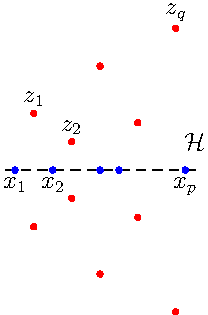
\includegraphics{C1622_1.pdf}
 \caption{Racines complexes d'un polynôme à coefficients réels}
 \label{fig:C1622_1}
\end{figure}

\begin{rem}
 On peut donc regrouper par deux les racines non réelles. Il est commode de repérer chaque couple par l'élément qui est dans le demi-plan $\mathcal H$ (dit de Poincaré) \index{demi plan de Poincaré} formé par les complexes de partie imaginaire strictement positive.
\end{rem}

\index{polynômes irréductibles de $\R[X]$}
\begin{prop}[Polynômes réels irréductibles]
Les polynômes irréductibles de $\R[X]$ sont les polynômes de degré $1$ et les polynômes de degré $2$ sans racine réelle.
\end{prop}
\begin{rem}
 Le polynome réel de degré 2 dont les racines sont des complexes non réels $z$ et $\overline{z}$ est
\begin{displaymath}
 (X-z)(X-\overline{z})=X^2 - 2\Re(z)X+|z|^2
\end{displaymath}
\end{rem}


\index{Décomposition en facteurs irréductibles dans $\R[X]$}
\begin{prop}[Décomposition des polynômes réels en facteurs irréductibles réels]
 La décomposition en facteurs irréductibles d'un polynôme $P$ à coefficients réels est de la forme suivante.
\begin{displaymath}
 P = \lambda \prod_{k=1}^p(X-x_k)^{m_k}\prod_{k=1}^q(X^2 - 2\Re(z_k)X+|z_k|^2)^{n_k}
\end{displaymath}
où $\lambda\in \R$ est le coefficient dominant de $P$, où les $x_k$ sont les racines réelles de $P$ et $m_k$ la multiplicité de $x_k$, où les $z_k$ sont les racines de $P$ dans $\mathcal H$ et $n_k$ la multiplicité de $z_k$.
\end{prop}

\section{Interpolation de Lagrange}
\index{polynômes d'interpolation de Lagrange}
\begin{defi}
 Soit $(x_1, \cdots, x_n)$ des éléments distincts de $\K$. les \emph{polynômes d'interpolation de Lagrange} sont les polynômes $(L_1, \cdots ,L_n)$ définis par
\[
\forall i \in \llbracket 1,n\rrbracket; L_i =
\frac{\prod_{k \in \llbracket 1,n \rrbracket \setminus \left\lbrace i\right\rbrace }(X-x_k)}
     {\prod_{k \in \llbracket 1,n \rrbracket \setminus \left\lbrace i\right\rbrace }(x_i-x_k)}
\]
\end{defi}
\begin{prop}
 Les polynômes d'interpolation de Lagrange attachés à $(x_1,\cdots, x_n)$ sont de degré $n-1$. De plus
\[
 \forall (i,j)\in \llbracket 1,n \rrbracket^2, \hspace{0.5cm}
\widetilde{P_i}(x_j) = \delta_{i,j}
=
\left\lbrace 
\begin{aligned}
 1 &\text{ si } i= j\\ 0 &\text{ si } i \neq j
\end{aligned}
\right. 
\]
\end{prop}
\begin{demo}
 à compléter.
\end{demo}
\index{symbole de Kronecker}
\begin{rem}
 $\delta_{i,j}$ est appelé le symbole de Kronecker.
\end{rem}

\begin{prop}
 Soit $(x_1, \cdots, x_n)$ des éléments distincts de $\K$ et $(y_1,\cdots, y_n)$ des éléments quelconques de $\K$. Il existe un unique $P\in \K_{n-1}[X]$ tel que
\[
 \forall i \in \llbracket 1,n \rrbracket,\hspace{0.5cm} \widetilde{P}(x_i) = y_j.
\]
Ce polynôme est appelé le polynôme interpolateur des $y_i$ aux $x_i$. Il est égal à
\[
 \sum_{k=1}^n y_yP_k.
\]

\end{prop} 
\begin{demo}
 à compléter
\end{demo}

\begin{prop}
 Soit $(x_1, \cdots, x_n)$ des éléments distincts de $\K$ et $(y_1,\cdots, y_n)$ des éléments quelconques de $\K$. Soit $P\in \K_{n-1}[X]$ le polynôme interpolateur. Alors, pour tout $Q\in \K[X]$:
\[
 \left( \forall i \in \llbracket 1,n \rrbracket,\hspace{0.5cm} \widetilde{Q}(x_i) = y_j\right) 
 \Leftrightarrow
 \left( \exists \Lambda \in \K[X] \text{ tq } Q = P + \Lambda \prod_{k=1}^n (X-x_k).
 \right) 
\]
Ce polynôme est appelé le polynôme interpolateur des $y_i$ aux $x_i$.
\end{prop} 
\begin{demo}
 à compléter
\end{demo}

\end{document}

